\documentclass[12pt]{article}
\usepackage[utf8]{inputenc}
\usepackage[cm]{fullpage}
\usepackage{amssymb}
\usepackage{multicol}
\usepackage{graphicx}

\usepackage{pgffor}   % for 'for loop' usage

\usepackage{pstricks}

\newcommand{\exerc}[3]{ \vspace{5pt} {$\mathbf{#1)}$} #2 \hfill {\it #3} }
\newcommand{\exitem}[2]{ \texttt{\bf #1)} #2 \\ }

%\newcommand{\clock}[1]{
%    \psset{yunit=0.8}
%	\rput(0,0.1){
%      \foreach \n in {0,...,#1}{
%	  \translate(2,0)
%      \psline
%	    (0,0)(1,0)(1,1)(2,1)
%	  }
%	}
%    \psset{yunit=1.0}
%}

%\newcommand{\signalBlock}[1]{
%  \vspace*{20pt}
%  \hspace*{-30pt}
%  \pscustom[xunit=0.5]{
%    \rput(1,2){#1}
%  }
%}

%\newcommand{\signal}[1]{
%    \psset{yunit=0.8}
%	\rput(0,0.1){
%    \psline
%	  #1
%	  }
%    \psset{yunit=1.0}
%}

\renewcommand{\neg}[1]{ 
  \mkern 1.5mu\overline{\mkern-1.5mu#1\mkern-1.5mu}\mkern 1.5mu
}

\newenvironment{exitems}[1]{
\\
\hspace*{30pt}
\begin{minipage}{0.8\textwidth}
\begin{multicols}{#1} 
}{
\end{multicols}
\end{minipage}
}

\newenvironment{exitemss}[1]{
\\
\hspace*{30pt}
\begin{minipage}{0.8\textwidth}
#1
}{
\end{minipage}
}

\begin{document}

\pagenumbering{gobble}

\begin{center}
{\Large \bf Elementos de Lógica Digital - 2015/2}
\end{center}

\vfill

{\large \bf 1ª Lista de exercícios}

{\bf dia:} 24/09/2015

\exerc{1}{Converter para o sistema decimal os seguintes números:}{}
\begin{exitems}{2}
	\exitem{a}{ $11100001_2$ }
	\exitem{b}{ $1011,110_2$ }
	\\
	\exitem{c}{ $19_{16}$ }
	\exitem{d}{ $4$CE$_{16}$ }
\end{exitems}

\exerc{2}{Converter para o sistema binário os seguintes números:}{}
\begin{exitems}{2}
	\exitem{a}{ $1573_{10}$ }
	\exitem{b}{ $565,69_{10}$ }
	\\
	\exitem{c}{ BA$_{16}$ }
	\exitem{d}{ C$7_{16}$ }
\end{exitems}

\exerc{3}{Converter para o sistema hexadecimal os seguintes números:}{}
\begin{exitems}{2}
	\exitem{a}{ $142_{10}$ }
	\exitem{b}{ $254_{10}$ }
	\\
	\exitem{c}{ $0110~1010~1110_2$ }
	\exitem{d}{ $1011~0100~1011_2$ }
\end{exitems}

\exerc{4}{Realize as seguintes operações utilizando a representação em
  complemento de 2:}{}
\begin{exitems}{2}
  \exitem{a}{ $142_{10} -078_{10}$ }
  \\
  \exitem{b}{ $131_{10} -052_{10}$ }
\end{exitems}

\exerc{5}{Simplifique as expressões utilizando álgebra de Boole:}{}
\begin{exitemss}
  \exitem{a}{ $\neg{A}\neg{B}\neg{C} + A\neg{B}\neg{C} + AB\neg{C} + ABC + \neg{A}\neg{B}C + A\neg{B}C$ }
  \exitem{b}{ $(B + \neg{C} + \neg{A}B)(BC + A\neg{B} + AC)$ }
  \exitem{c}{ $\neg{(A+\neg{B} + \neg{C})} + \neg{(C + \neg{A} + C)} + \neg{(A + \neg{B} + C)}$ }
\end{exitemss}

\exerc{6}{Implemente circuitos que executem as expressões encontradas no exercício anterior, utilizando apenas portas NAND.}

\exerc{7}{Projete um circuito que realiza a subtração de números binários de 4 dígitos.}{}

\exerc{8}{ Esboçe a forma de onda da saída "Q" do flip-flop dado os sinais abaixo:}
\\
\begin{multicols}{2}
\begin{center}
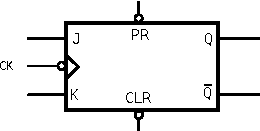
\includegraphics{fp-jk} \\ \vspace{15pt}
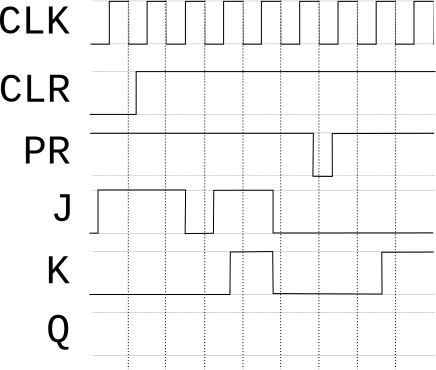
\includegraphics[scale=0.5]{sig1} \\
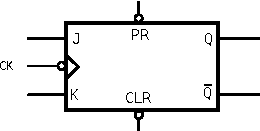
\includegraphics{fp-jk} \\ \vspace{15pt}
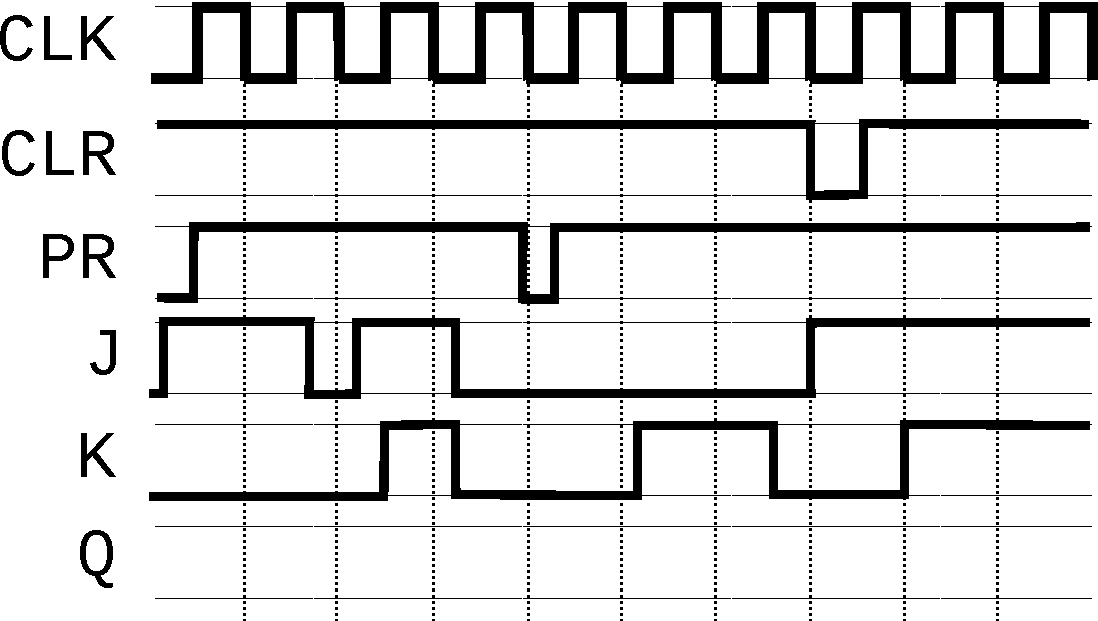
\includegraphics[scale=0.5]{sig2}
\end{center}
\end{multicols}

\end{document}

